\section{Fields}
Fields are implemented in the system, as JSON fields on instances of the \textit{Asset} and \textit{Tag} classes. The fields are used to customize the information saved on specific assets and tags. The field class contains the information seen in \autoref{fig:FieldClass}. The type is specified as a enum, which is used to define the field type, there are Textarea, TextBox, NumberField, Date and Checkbox. The field types are used to define the way the field is presented visually, as well as the content that can be saved in the field. The field itself is not stored as its own instance in a database, but is instead serialized and saved unto the \textit{Asset} or \textit{Tag} itself.

\begin{figure}[H]
    \centering
    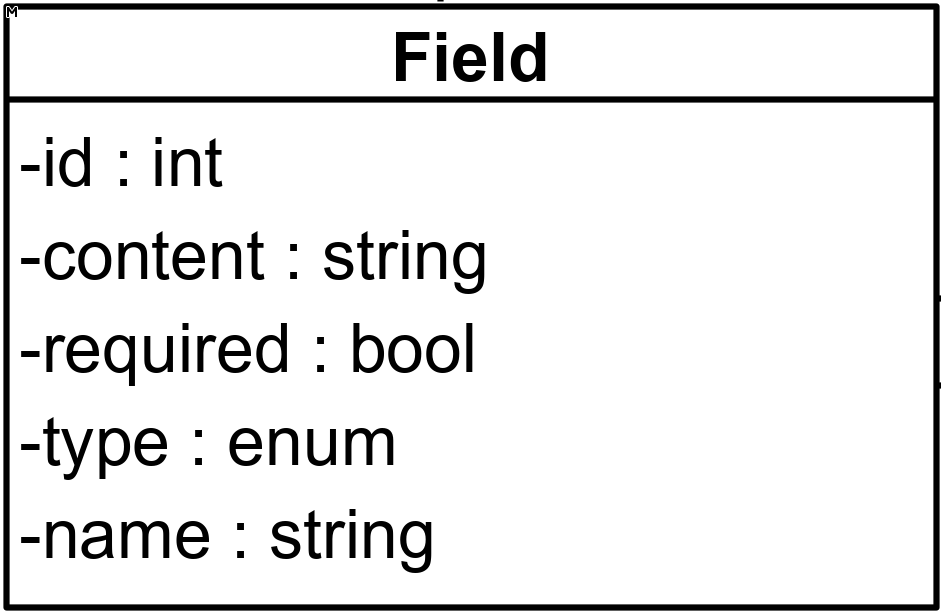
\includegraphics[width=0.5\textwidth]{figures/FieldClass.PNG}
    \caption{Field class}
    \label{fig:FieldClass}
\end{figure}